\section{DataProfilingTaskSample}
\subsection{Datenquellenbeschreibung}
\DqBeschreibung{DataProfilingTaskSample}{Ein einfache Datenquelle, die zum Testen gebaut habe}{csv}
\Quellattribut{ID}{Fortlaufende ID}
\Quellattribut{Geschlecht} {In der Kodierung m und w}
\Quellattribut{Alter}{Alter als numerischer String. Werte sollen zwischen 0 und 130 liegen}
\Quellattribut{Vermögen}{Numerischer Ganzzahl String}



\subsection{Extraktion}
Hier wird mittels csv flatfile Import realisiert
\subsection{Kodierung}
\subsection{Vollst"andigkeit und Struktur}
Die Vollst"andigkeit und die Struktur wird in dem Paket \SsisPack{Bereinigung.dtsx} realisiert. Und ist in der Abbildung  dargestellt. Zuerst wird auf leere oder null-Werte überprüft und aussortiert. Dies passiert im Task \SsisTask{CheckNullOrEmptyColumns}. Haben Zeilen leere Werte, werden diese komplett aussortiert und in die Tabelle eingefügt\\

Die L"ange der Datentypen und die Formatieren werden im Task \SsisTask{Length and type Check} ausgeführt. Hier wird die L"ange des Geschlecht und ob es sich bei Alter um eine Zahl handelt.

\paragraph{SISS Paket}
\begin{figure}
	\centering
		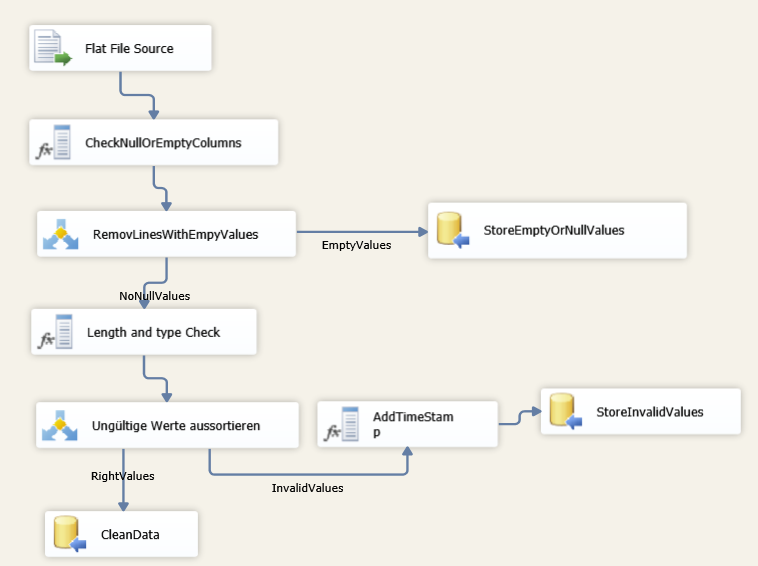
\includegraphics[width=1.00\textwidth]{doku/Bilder/DataProfilingTaskSampleVollstaendigkeitUndStrukturSISS.PNG}
	\caption{Vollst"andigkeit und Struktur SISS Paket}
	\label{fig:DataProf}
\end{figure}
\paragraph{Verwendete Logging Tabellen}
\begin{figure}
	\centering
		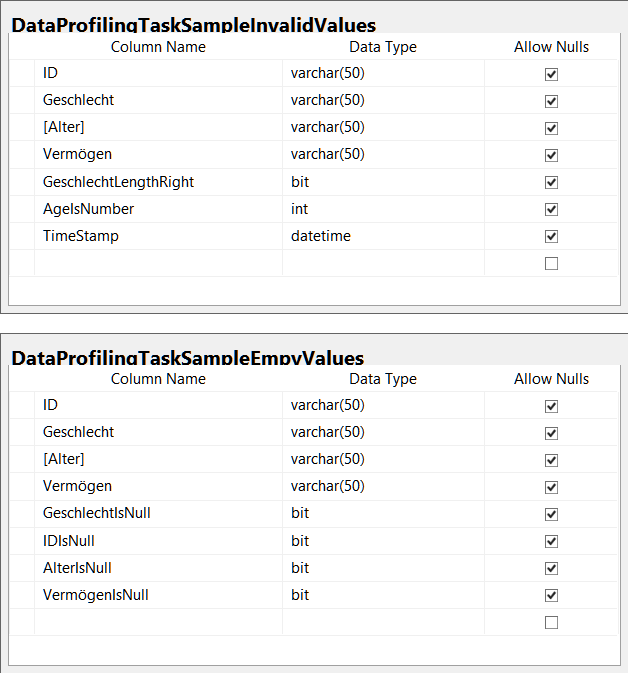
\includegraphics[width=0.70\textwidth]{doku/Bilder/LoggingTables.png}
	\caption{Logging Tabellen}
	\label{fig:LoggingTables}
\end{figure}



\subsection{Umsetzung Fachlichkeit} Hier muss die Regel \ref{Rule:WertebereichAlter} Anwendung finden, da ... Realisiert wurde dies mit der SSIS Komponente \SsisTask{Fachliche Regel Alter}
\begin{lstlisting}
(DT_I4)Alter >= 0 && (DT_I4)Alter <= 130
\end{lstlisting}
